
\chapter{INTRODUÇÃO}
\label{chap:introducao}

% INTRODUÇÃO-------------------------------------------------------------------

O e-commerce, que em português significa comércio eletrônico, é uma modalidade de comércio que realiza suas transações financeiras por meio de dispositivos e plataformas eletrônicas, como computadores e celulares. Um exemplo deste tipo de comércio é comprar ou vender produtos em lojas virtuais. 
No início, o e-commerce era utilizado basicamente para vender bens tangíveis com valores modestos, como: livros e CDs. Hoje, ele é utilizado para comercializar desde produtos que custam milhões, como: iates, carros de luxo e mansões, até produtos que há pouco tempo eram inimagináveis pela sua incompatibilidade com este tipo de comércio, como roupas, perfumes e alimentos. \cite{ecomm} %%ver data da postagem no site??

%%% Verifica a inserção desta parte no trabalho. 
%Segundo \cite{gestcont}, o e-commerce permite que os consumidores transacionem bens e serviços eletronicamente sem barreiras de tempo ou distância.

Sabe-se que atualmente está sendo mais frequente o uso de lojas virtuais para realizar compras sem ser necessário fazer a locomoção para poder adquirir o produto desejado. Pensando no crescimento do comércio eletrônico, foi proposto no presente trabalho o desenvolvimento de um e-commerce voltado para moda, roupas e acessórios. 

Este trabalho será desenvolvido utilizando a linguagem de programação PHP juntamento com o framework codeigniter, juntamente com CSS, HTML, Javascript e  utilizando banco de dados MySql.
No decorrer das aulas foi realizada a documentação do trabalho contendo a explicação sobre o diagrama UML, sendo compreendido e relatado nos seguintes capítulos descritos abaixo.

No primeiro capítulo é relatado as linguagens que serão utilizadas no decorrer do desenvolvimento do sistema.

No segundo, descrito os diagramas de casos de uso e suas descrições.

No terceiro capítulo trata-se da modelagem conceitual contendo o diagrama de classes juntamente com a identificação entre essas classes.

No quarto capítulo foi construindo também os diagramas de sequência e diagrama de atividades.


\chapter{ESCOPO}
\label{chap:escopo}

O seguinte projeto possui página principal que irá conter informações referentes à história do site, menu para pesquisa de itens, uma sacola para adicionar os produtos, como roupas e acessórios escolhidos durante a compra.

\chapter{TECNOLOGIAS UTILIZADAS}
\label{chap:tec}

O trabalho foi planejado para ser desenvolvido com as seguintes linguagens abaixo, sendo que como o projeto ainda não foi iniciado, está possível de ser alterado qualquer uma das citadas abaixo.

\section{HTML}
 \textit{HTML} é uma das linguagens que utilizamos para desenvolver websites. O acrônimo HTML vem do inglês e significa Hypertext Markup Language ou em português Linguagem de Marcação de Hipertexto.

O HTML é a liguagem base da internet. Foi criada para ser de fácil entendimento por seres humanos e também por máquinas, como por exemplo o Google ou outros sistemas que percorrem a internet capturando informação.\cite{html}

\section{CSS}
O Cascading Style Sheets  (\textit{CSS}) é uma "folha de estilo" composta por “camadas” e utilizada para definir a apresentação (aparência) em páginas da internet que adotam para o seu desenvolvimento linguagens de marcação (como  \textit{XML, HTML e XHTML}). O CSS define como serão exibidos os elementos contidos no código de uma página da internet e sua maior vantagem é efetuar a separação entre o formato e o conteúdo de um documento. \cite{css1}.

Quando falamos de acessibilidade, performance e manutenção, tem-se como princípio fazer separação do conteúdo, da interatividade e da apresentação de um site ou aplicação web. O CSS desempenha um grande papel na camada da apresentação.
A forma certa de publicar um documento web é seguindo uma estrutura semântica. O CSS traz toda a informação do layout, isto é, cores, posicionamento, fontes, tamanhos e imagens de fundo, enquanto o HTML deve fornecer uma “arquitetura” para o conteúdo. O suporte a CSS pelos navegadores de hoje é bem sólido, mas teve um início tímido, sendo inicialmente suportado pelo navegador Netscape. \cite{css2}

\section{PHP}

A sigla  \textit{PHP} vem do inglês Personal Home Page que traduzido para o português significa página pessoal principal. Normalmente as páginas web são feitas com código de hipertexto (um código que permite a ligação de palavras a outros sites da internet ou a outros da mesma página). No caso da PHP este código pode ser encontrado no código HTML ou hipertexto

O PHP é um código usado por ser fácil de aprender e ainda por cima grátis. Muita gente aprende porque é muito solicitado na criação de páginas web corporativas e pessoais, no entanto, é necessário certo conhecimento básico de informática, especialmente de código HTML. Ele pode ser incorporado obrigatoriamente aos servidores de página web e produzir animações, efeitos variados de cores, movimentos de certos elementos, etc. Seus efeitos visuais podem ser desde muito simples até animações bem complexas, da mesma forma das que aparecem às vezes na página principal do Google. \cite{php}

\section{MySQL}

O  \textit{MySQL} é um sistema gerenciador de banco de dados relacional de código aberto usado na maioria das aplicações gratuitas para gerir suas bases de dados. O serviço utiliza a linguagem  \textit{SQL}x' (Structure Query Language – Linguagem de Consulta Estruturada), que é a linguagem mais popular para inserir, acessar e gerenciar o conteúdo armazenado num banco de dados.
a criação de aplicações web abertas e gratuitas, o conjunto de aplicações mais usado é o LAMP, um acrônimo para Linux, Apache, \textit{MySQL e Perl/PHP/Python}. Nesse conjunto de aplicações, inclui-se, respectivamente, um sistema operacional, um servidor web, um sistema gerenciador de banco de dados e uma linguagem de programação. Assim, o MySQL é um dos componentes centrais da maioria das aplicações públicas da Internet. \cite{mysql}

%%%%%%%%%%%%%%%%%%%%%%______________________________%%%%%%%%%%%%%%%%%%%%%%______________________________%%%%%%%%%%%%%%%%%%%%%%______________________________


\chapter{DIAGRAMA UML}
\label{chap:diauml}
A \textit{UML}, Unified Modeling Language ou Linguagem de Modelagem Unificada é uma linguagem visual utilizada para modelar softwares baseados no paradigma de orientação a objetos. A linguagem pode ser aplicada a todos os domínios de aplicação pois possui um propósito geral e se tornou, nos últimos anos, a linguagem padrão de modelagem adotada pelos engenheiros de software de todo o mundo \cite{Guedes}.

A UML apresenta as seguintes características principais:
É independente do domínio de aplicação, pode ser usado em projetos de diferentes características, tais como sistemas cliente/
servidor tradicionais; sistemas baseados na Web; sistemas de informação geográficos; sistemas de tempo real); é independente do processo ou metodologia de desenvolvimento; é independente das ferramentas de modelagem; apresenta mecanismos potentes de extensão; agrega um conjunto muito significativo de diferentes
diagramas/técnicas dispersos por diferentes linguagens, diagramas de casos de utilização, de classes, de objetos, de colaboração, de 
atividades, de estados, de componentes, e de instalação). \cite{Alberto}

\section{Análise de Requisitos}
\label{sec:anareq}
%%%%%%--------------------------------------------------------------------------------------------%%%%%%
\subsection{Definição dos Atores}
\label{sec:casuso}

\subsection{Casos de Uso}
\label{sec:casuso}
Diagrama de casos de uso é um diagrama muito importante de ser utilizado devido às vantagens que se pode ter, pensando na possibilidade de desenvolver um sistema voltado para um cliente. Esses diagramas são muito claros e visíveis para o usuário explicar o que ele realmente deseja que o sistema faça, e sendo fácil para o analista de projeto fazer a análise das informações com mais clareza.

\begin{figure}[H]
    \centering
    \caption{Diagrama de Caso de Uso -  Realizar Compra}
    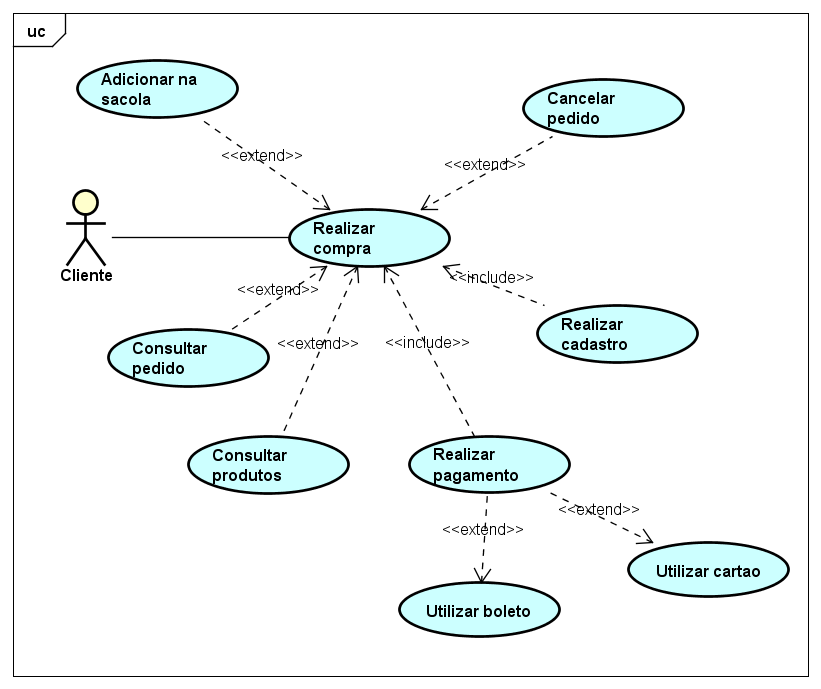
\includegraphics[width=1.0\textwidth]{./dados/figuras/4_1}
    \fonte{Autor}
    \label{fig:figura-1}
\end{figure}
\begin{figure}[H]
    \centering
    \caption{Diagrama de Caso de Uso - Realizar Cadastro}
    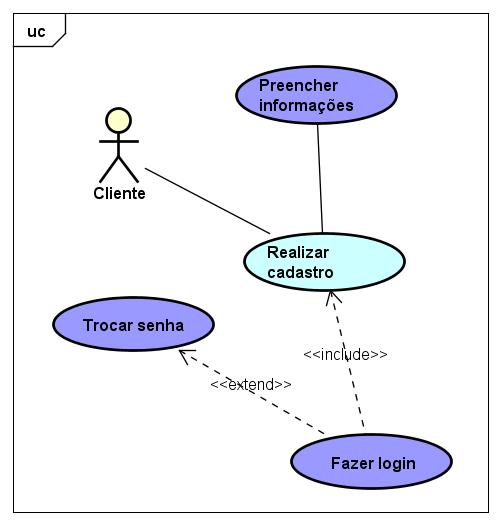
\includegraphics[width=1.0\textwidth]{./dados/figuras/3}
    \fonte{Autor}
    \label{fig:figura-1}
\end{figure}
%%%%%%--------------------------------------------------------------------------------------------%%%%%%
\subsection{Descrição dos Casos de Uso}
\label{sec:conuso}

\begin{figure}[H]
    \centering
    \caption{Descrição do Caso de Uso -  Realizar Compra}
    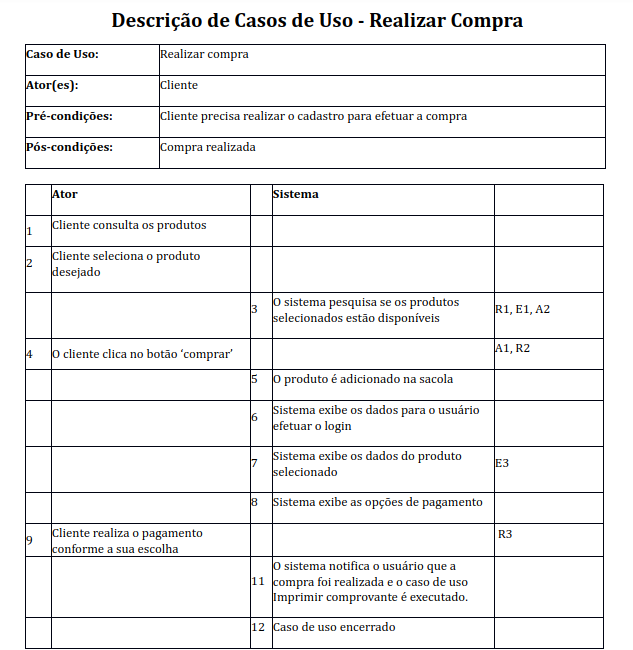
\includegraphics[width=1.0\textwidth]{./dados/figuras/1}
    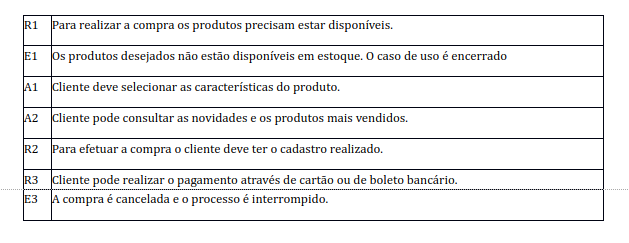
\includegraphics[width=1.0\textwidth]{./dados/figuras/1_2}
    \fonte{Autor}
    \label{fig:figura-1}
\end{figure}
\begin{figure}[H]  %!htb
    \centering
    \caption{Descrição do Caso de Uso -  Realizar Cadastro}
    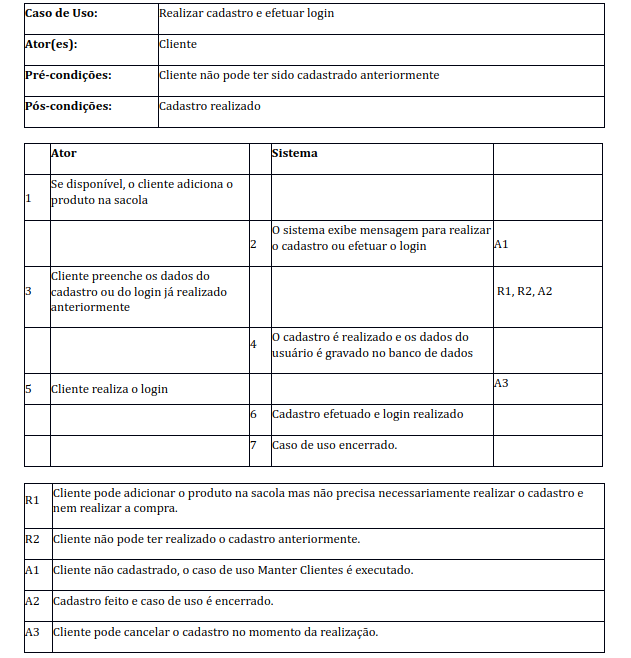
\includegraphics[width=1.0\textwidth]{./dados/figuras/2}
    \fonte{Autor}
    \label{fig:figura-1}
\end{figure}


%%%%%%--------------------------------------------------------------------------------------------%%%%%%

\section{Modelagem Conceitual}
\label{sec:modcon}

\subsection{Diagrama de Classes de Análise}
\label{sec:diacla}
\begin{figure}[H]
    \centering
    \caption{Diagrama de Classe}
    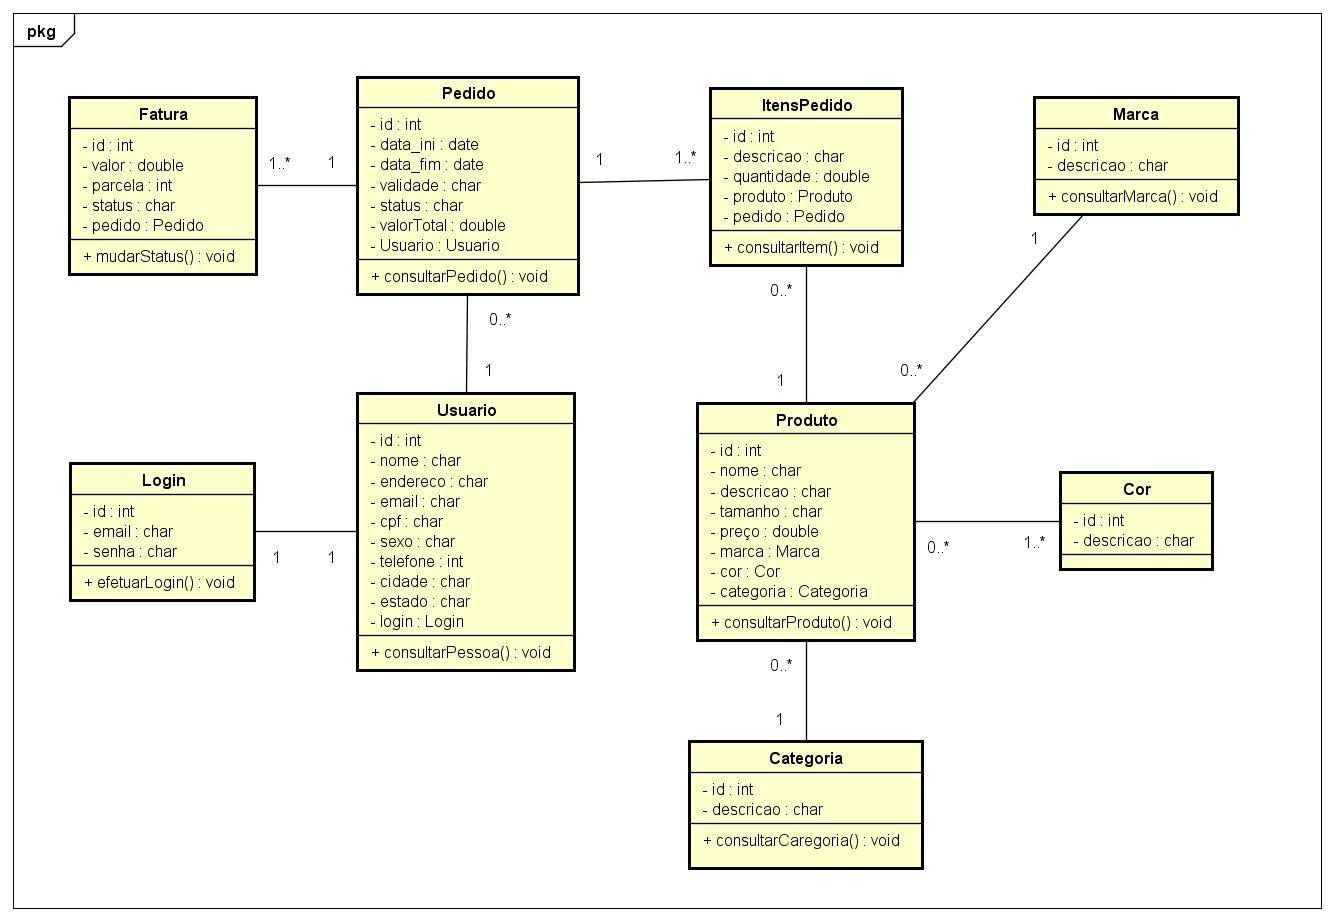
\includegraphics[width=1.0\textwidth]{./dados/figuras/5}
    \fonte{Autor}
    \label{fig:figura-1}
\end{figure}
%%%%%%%%%%%%%%%%%%%%%%%%%%%%%%%%%%%%%%%%%%%%%%%%%%%%%%%%%%%%%%%%%%
\section{Modelagem comportamental}
\label{sec:modcom}

\subsection{Construção dos Diagramas de Sequência}
\label{sec:conseq}

\begin{figure}[H]
    \centering
    \caption{Diagrama de Sequência - Fazer Login}
    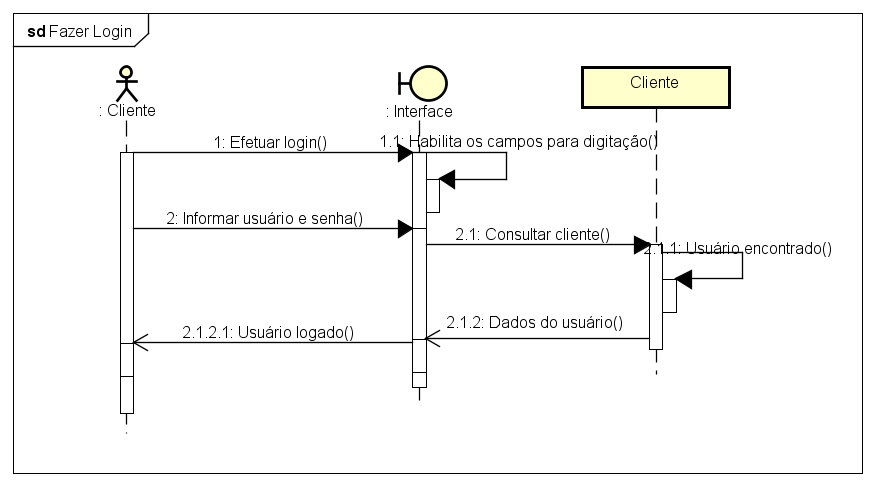
\includegraphics[width=1.0\textwidth]{./dados/figuras/7}
    \fonte{Autor}
    \label{fig:figura-1}
\end{figure}
\begin{figure}[H]
    \centering
    \caption{Diagrama de Sequência - Realizar Cadastro}
    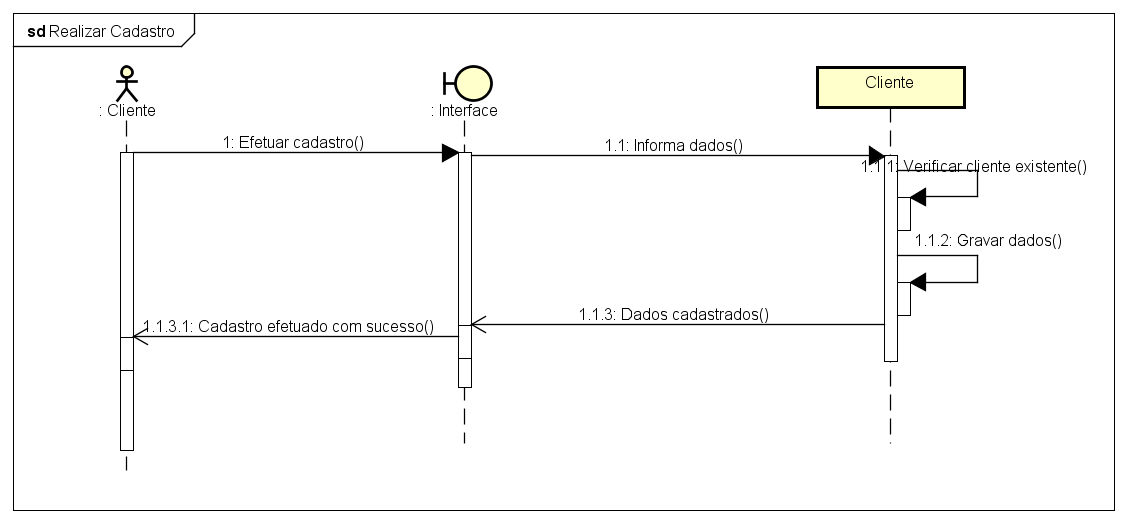
\includegraphics[width=1.0\textwidth]{./dados/figuras/8}
    \fonte{Autor}
    \label{fig:figura-1}
\end{figure}
\begin{figure}[H]
    \centering
    \caption{Diagrama de Sequência - Realizar Compra}
    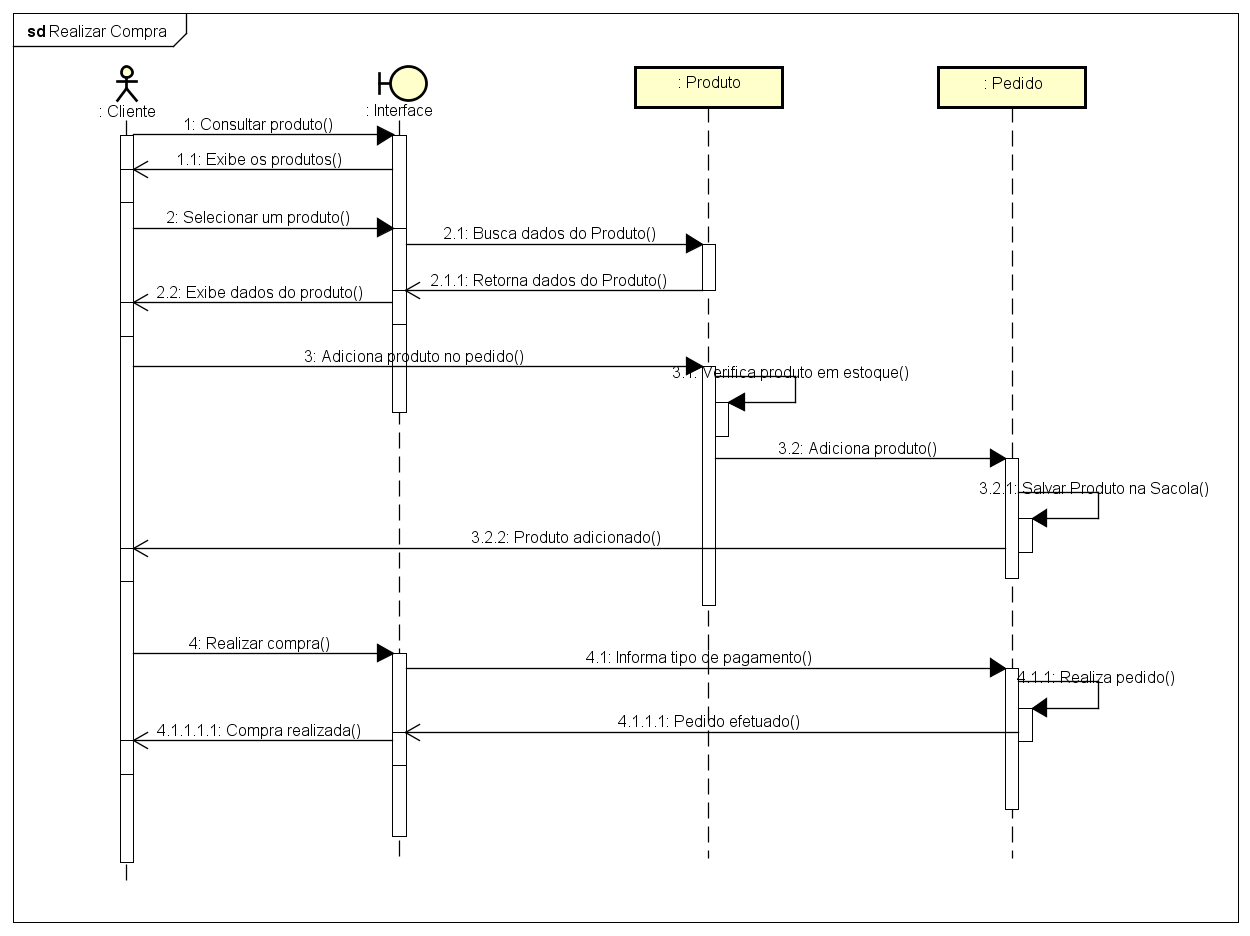
\includegraphics[width=1.0\textwidth]{./dados/figuras/9}
    \fonte{Autor}
    \label{fig:figura-1}
\end{figure}

%%%%%%%%%%%%%%%%%%%%%%%%%%%%%%%%%%%%%%%%%%%%%%%%%%%%%%%%%%%%%%%%%%
\subsection{Construção do Diagrama de Atividade}
\label{sec:diaati}

\begin{figure}[H]
    \centering
    \caption{Diagrama de Atividade}
    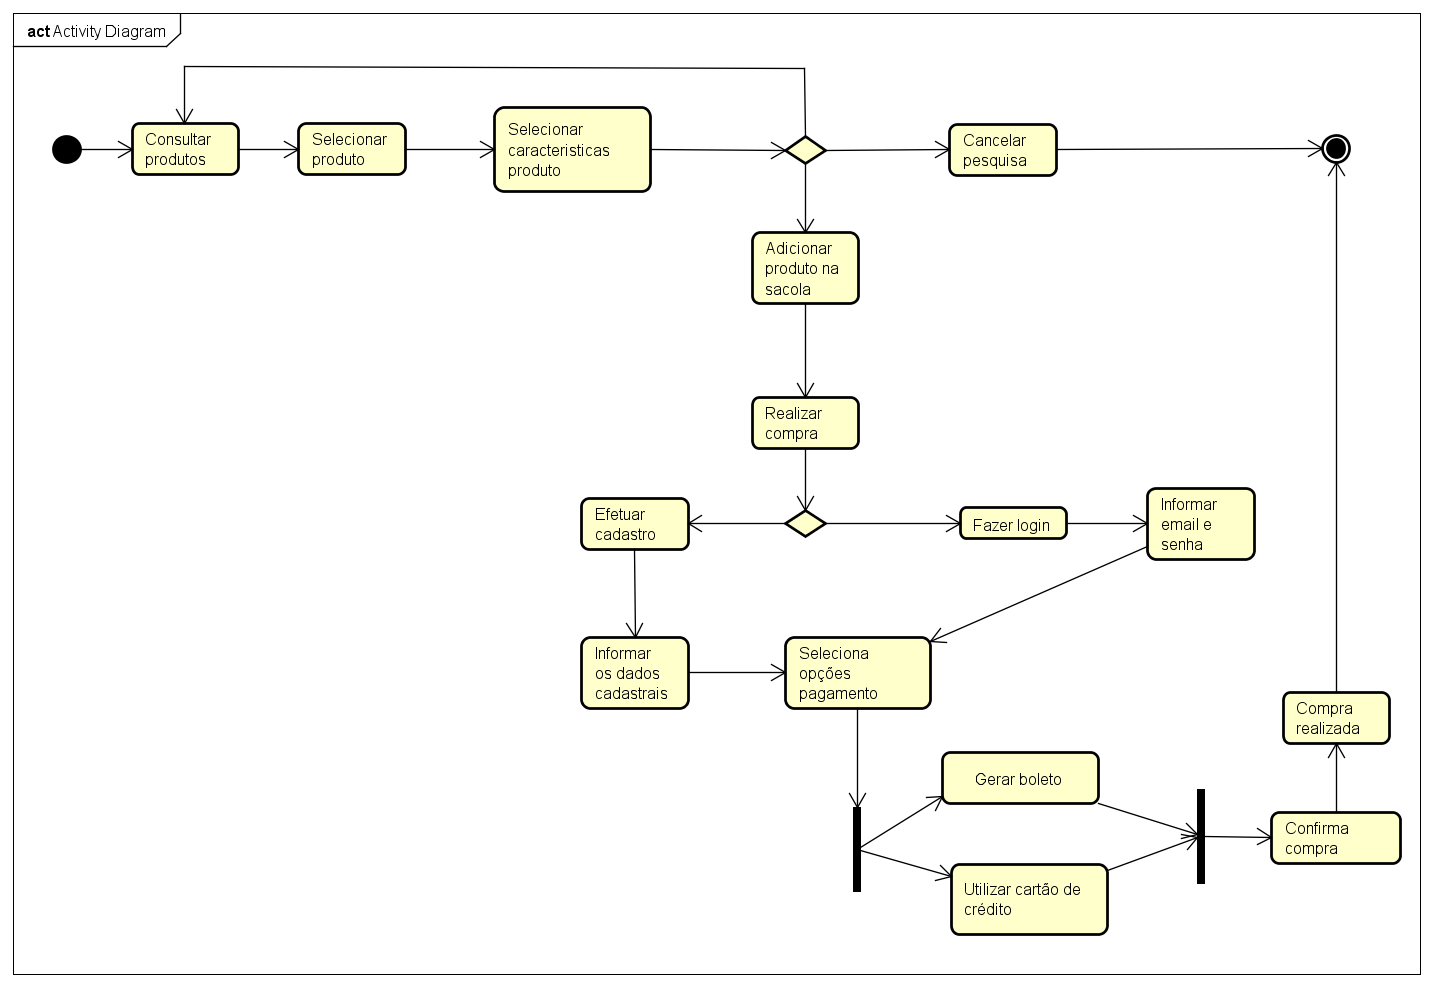
\includegraphics[width=1.0\textwidth]{./dados/figuras/6}
    \fonte{Autor}
    \label{fig:figura-1}
\end{figure}

%-----------------------------------------------------------------------------------------------------------